\documentclass[10pt,french]{book}
\input preambule_2013
\input philippe2013_activites
\pagestyle{empty}

\begin{document}

\TitreActivite{v.4}{Utilisation d'un\par tableau de variations}

\exo Soit $f$ la fonction définie par sa courbe représentative et son tableau de variation :

\begin{center}
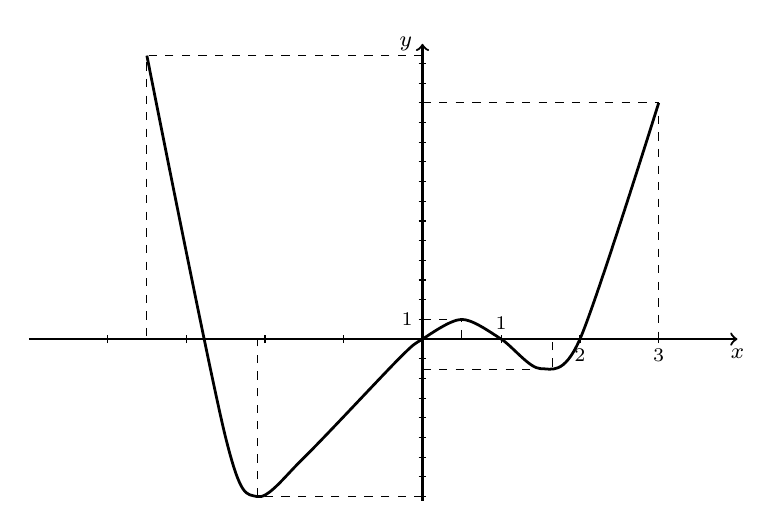
\begin{tikzpicture}[yscale=0.25]
    %\draw[gray] (-4,-8)grid(4,15);
    \draw[thick,->] (-5,0)--(4,0)node[below] {\footnotesize $x$};
    \draw[thick,->] (0,-8.2)--(0,15)node[left] {\footnotesize $y$};
    \draw[line width=1pt] plot[smooth=200] coordinates{(-3.5,14.4)(-2.5,-5)(-2.1,-8)(-1.5,-6)(-0.3,-1)(0,0)(0.5,1)(1,0)(1.5,-1.5)(2,0)(3,12)};
    \draw[dashed] (0,-1.55)-|(1.65,0);
    \draw[dashed] (0,14.4)-|(-3.5,0);
    \draw[dashed] (0,-8)-|(-2.1,0);
    \draw[dashed] (0,1)-|(0.5,0);
    \draw[dashed] (0,12)-|(3,0);
    \foreach \x in {-4,...,3} \draw (\x,-0.2)--(\x,0.2);
    \foreach \x in {-8,...,14} \draw (-0.05,\x)--(0.05,\x);
     \draw (1,0) node[above] {\scriptsize $1$};\draw (2,0) node[below] {\scriptsize $2$};
     \draw (3,0) node[below] {\scriptsize $3$};\draw (0,1) node[left] {\scriptsize $1$};
\end{tikzpicture}
\end{center}

\begin{center}
\begin{tikzpicture}
\small
    \tkzTabInit[nocadre,lgt=2.5,espcl=2.5]{$x$/1,Variations de \\ $f(x)$/2}{{$-3,5$},{$-2,1$},{$0,5$},{$1,65$},$3$}
    \tkzTabVar{+/{$14,4$},-/$-8$,+/{$1$},-/{$-1,55$},+/$12$}
\end{tikzpicture}
\end{center}

\begin{enumerate}
    \item Donner l'ensemble de définition de la fonction $f$.
    \item Déterminer les images par $f$ des nombres $-2,1 \pv 0$ et $3$.
    \item Trouver les antécédents de $0$ par $f$.
    \item Résoudre graphiquement l'inéquation $f(x) \leqslant 0$.
    \item Construire le tableau de signes de la fonction $f$.
\end{enumerate}

\exo On considère le tableau de variation suivant :
\begin{center}
\begin{tikzpicture}
\small
    \tkzTabInit[nocadre,lgt=2.5,espcl=1.5]{$x$/1,Variations de \\ $g(x)$/2}{$-4$,$-2$,,,$3$,,$6$}
    \tkzTabVar{+/$3$,-/{$-5,5$},R,R,+/{$8,5$},R,-/{$-7$}}
    \tkzTabVal{2}{5}{0.33}{$0$}{$-1$}
    \tkzTabVal{2}{5}{0.66}{$1$}{$3$}
    \tkzTabVal{5}{7}{0.5}{$5$}{$3$}
\end{tikzpicture}
\end{center}

\begin{enumerate}
    \item Tracer une courbe susceptible de représenter la fonction $g$.
    \item En rédigeant convenablement, comparer les nombres suivants :
        \[g(1) \text{ et } g(2) \qq g(4) \text{ et } g(5,5) \qq g(-3) \text{ et } g(2) \qq g(0,5) \text{ et } g(4) \qq g(4,5) \text{ et } 2\]
    \item Trouver le signe des nombres suivants :
        \[g(2) \qq g(4) - 3 \qq g(3,5) - g(5,5) \qq g\left(\sqrt 7\right) - 9.\]
\end{enumerate}
\end{document}
